% Chapter 3: Methodology and System Design
\chapter{Methodology and System Design}
\label{chap:methodology}

\section{Research Approach}
\label{sec:research-approach}
This chapter presents our systematic approach to developing an ontology-enhanced LLM system for STEM education. Our methodology addresses the critical challenge of AI hallucination in educational applications through the following research objectives:

\begin{itemize}
    \item Integration of domain-specific ontologies (OWL, RDF, SPARQL) with LLM reasoning \cite{doubletaken2024llm}
    \item Development of mechanisms for reliable AI-powered tutoring \cite{ji2023survey}
    \item Enhancement of contextual understanding in STEM education through structured knowledge representation
    \item Creation of an adaptive, personalized learning system with avatar-based engagement
\end{itemize}

The research follows a phased development approach focusing on three key areas:
\begin{enumerate}
    \item \textbf{Core Functionality:} Environment setup, API authentication, system prompt structure, and basic question-answering functionality
    \item \textbf{Knowledge Representation:} Physics concepts, laws, relationships, prerequisites structures, and context retrieval system
    \item \textbf{Student Model Implementation:} Concept exposure tracking, knowledge level monitoring, and learning path generation
\end{enumerate}

\section{System Architecture}
\label{sec:system-architecture}

The system architecture comprises several interconnected components organized into distinct layers:

\begin{figure}[htbp]
    \centering
    % System Architecture Diagram using TikZ
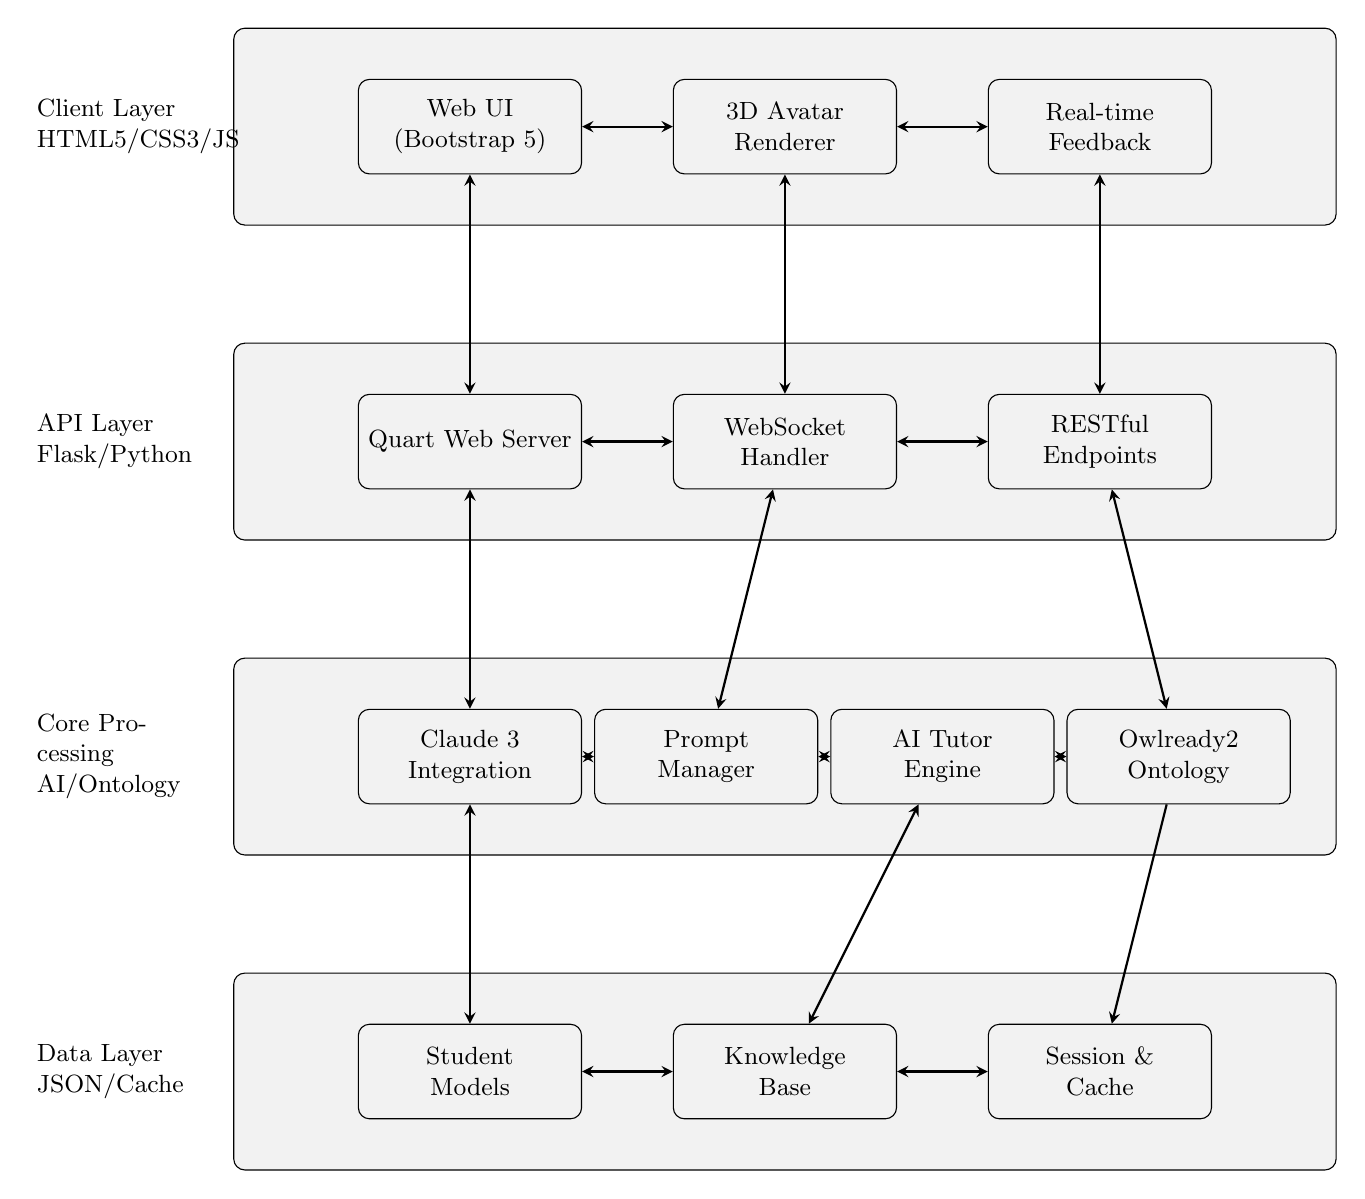
\begin{tikzpicture}[
    % Define styles for different node types
    box/.style={
        draw,
        rectangle,
        rounded corners,
        minimum width=2.8cm,
        minimum height=1.2cm,
        text centered,
        text width=2.6cm,
        font=\small
    },
    layer/.style={
        draw,
        rectangle,
        rounded corners,
        minimum width=14cm,
        minimum height=2.5cm,
        fill=gray!10
    },
    arrow/.style={
        ->,
        >=stealth,
        thick
    },
    bidirectional/.style={
        <->,
        >=stealth,
        thick
    },
    layer_label/.style={
        text width=3cm,
        align=left,
        font=\small
    }
]

% Define the layers with proper spacing
\begin{scope}[shift={(0,0)}]
    % Layer background rectangles with adjusted spacing
    \node[layer] (client) at (0,12) {};
    \node[layer] (api) at (0,8) {};
    \node[layer] (core) at (0,4) {};
    \node[layer] (data) at (0,0) {};

    % Layer labels on the left with better spacing
    \node[layer_label] at (-8,12) {Client Layer\\HTML5/CSS3/JS};
    \node[layer_label] at (-8,8) {API Layer\\Flask/Python};
    \node[layer_label] at (-8,4) {Core Pro-\\cessing\\AI/Ontology};
    \node[layer_label] at (-8,0) {Data Layer\\JSON/Cache};

    % Client Layer Components with even spacing
    \node[box] (browser) at (-4,12) {\parbox{2.6cm}{\centering Web UI\\(Bootstrap 5)}};
    \node[box] (avatar) at (0,12) {\parbox{2.6cm}{\centering 3D Avatar\\Renderer}};
    \node[box] (frontend) at (4,12) {\parbox{2.6cm}{\centering Real-time\\Feedback}};

    % API Layer Components
    \node[box] (gateway) at (-4,8) {Quart Web Server};
    \node[box] (websocket) at (0,8) {\parbox{2.6cm}{\centering WebSocket\\Handler}};
    \node[box] (endpoints) at (4,8) {\parbox{2.6cm}{\centering RESTful\\Endpoints}};

    % Core Processing Components with adjusted spacing
    \node[box] (llm) at (-4,4) {\parbox{2.6cm}{\centering Claude 3\\Integration}};
    \node[box] (prompt) at (-1,4) {\parbox{2.6cm}{\centering Prompt\\Manager}};
    \node[box] (tutor) at (2,4) {\parbox{2.6cm}{\centering AI Tutor\\Engine}};
    \node[box] (ontology) at (5,4) {\parbox{2.6cm}{\centering Owlready2\\Ontology}};

    % Data Layer Components
    \node[box] (student) at (-4,0) {\parbox{2.6cm}{\centering Student\\Models}};
    \node[box] (knowledge) at (0,0) {\parbox{2.6cm}{\centering Knowledge\\Base}};
    \node[box] (session) at (4,0) {\parbox{2.6cm}{\centering Session \&\\Cache}};

    % Vertical Connections
    \draw[bidirectional] (browser) -- (gateway);
    \draw[bidirectional] (avatar) -- (websocket);
    \draw[bidirectional] (frontend) -- (endpoints);

    \draw[bidirectional] (gateway) -- (llm);
    \draw[bidirectional] (websocket) -- (prompt);
    \draw[bidirectional] (endpoints) -- (ontology);

    \draw[bidirectional] (llm) -- (student);
    \draw[bidirectional] (tutor) -- (knowledge);
    \draw[arrow] (ontology) -- (session);

    % Horizontal Connections
    \draw[bidirectional] (browser) -- (avatar);
    \draw[bidirectional] (avatar) -- (frontend);
    \draw[bidirectional] (gateway) -- (websocket);
    \draw[bidirectional] (websocket) -- (endpoints);
    \draw[bidirectional] (llm) -- (prompt);
    \draw[bidirectional] (prompt) -- (tutor);
    \draw[bidirectional] (tutor) -- (ontology);
    \draw[bidirectional] (student) -- (knowledge);
    \draw[bidirectional] (knowledge) -- (session);
\end{scope}
\end{tikzpicture} 
    \caption{High-level System Architecture showing the integration of ontology-driven knowledge models with Claude 3 LLM for enhanced STEM education.}
    \label{fig:system-architecture}
\end{figure}

\subsection{Core Components}
\label{subsec:core-components}

The system consists of the following key components:

\begin{itemize}
    \item \textbf{Backend (API Layer):} 
        \begin{itemize}
            \item Quart (async Flask-compatible) server
            \item Modular API endpoints and route definitions
            \item JWT session management
            \item Integration with Claude 3 LLM and ontology modules
        \end{itemize}
    
    \item \textbf{LLM Integration:} \cite{vu2024freshllms}
        \begin{itemize}
            \item Adaptive tutoring logic
            \item Student model implementation
            \item Context-aware answer generation
            \item Response validation against ontology
        \end{itemize}
    
    \item \textbf{Ontology Layer:} \cite{mendel2024hypercubes}
        \begin{itemize}
            \item Physics domain ontology schemas
            \item Validation mechanisms
            \item Knowledge representation structures
            \item Semantic reasoning capabilities
        \end{itemize}
    
    \item \textbf{Frontend Interface:} 
        \begin{itemize}
            \item Avatar-based web UI
            \item Interactive tutoring interface
            \item Real-time feedback visualization
            \item Student progress tracking
        \end{itemize}
\end{itemize}

\section{Project Structure}
\label{sec:project-structure}

The implementation follows a modular organization:

\begin{itemize}
    \item \textbf{/api} 
        \begin{itemize}
            \item Routes and handler definitions
            \item Utility functions
            \item Main API application
            \item Vercel serverless handler
        \end{itemize}
    
    \item \textbf{/llm\_integration}
        \begin{itemize}
            \item LLM integration components
            \item Student modeling logic
            \item Context management
            \item Response generation
        \end{itemize}
    
    \item \textbf{/ontology}
        \begin{itemize}
            \item Physics ontology schemas
            \item Validation mechanisms
            \item Knowledge base structures
            \item Reasoning components
        \end{itemize}
    
    \item \textbf{/static}
        \begin{itemize}
            \item Frontend assets (HTML, CSS, JS)
            \item Avatar interface components
            \item UI/UX elements
            \item Interactive features
        \end{itemize}
\end{itemize}

\section{Evaluation Metrics}
\label{sec:evaluation-metrics}

The system evaluation is conducted across three primary dimensions \cite{huang2024survey}:

\begin{enumerate}
    \item \textbf{System Performance}
        \begin{itemize}
            \item Response accuracy measurement
            \item Personalization effectiveness
            \item System scalability assessment
            \item Integration reliability
        \end{itemize}
    
    \item \textbf{User Experience}
        \begin{itemize}
            \item Interaction quality metrics
            \item Learning engagement levels
            \item Knowledge retention rates
            \item Avatar interaction effectiveness
        \end{itemize}
    
    \item \textbf{Technical Evaluation}
        \begin{itemize}
            \item API integration performance
            \item Knowledge representation accuracy
            \item Data management efficiency
            \item Response validation success
        \end{itemize}
\end{enumerate}

\section{Research Contributions}
\label{sec:research-contributions}

The key contributions of this research include:

\begin{enumerate}
    \item \textbf{Reduced Hallucination:} Integration of structured domain knowledge to enhance AI accuracy \cite{su2024confabulation}
    \item \textbf{Personalized Tutoring:} Adaptive responses based on comprehensive student modeling
    \item \textbf{Scalable Solution:} Architecture supporting one-on-one tutoring at scale
    \item \textbf{Interactive Learning:} Avatar-based interface for enhanced student engagement
    \item \textbf{Knowledge Verification:} Systematic validation of AI responses against domain ontology \cite{scibite2024ontologies}
\end{enumerate}

This methodology provides a comprehensive framework for developing and evaluating our ontology-enhanced LLM system, ensuring alignment with our research objectives and educational goals. 